\documentclass{article}

\usepackage[a4paper,hmargin=1.2in,vmargin=1.5in]{geometry}
\usepackage[parfill]{parskip} % for distance between paragraphs
\usepackage{ragged2e} % for alignment
\usepackage{hyperref} % for link
\usepackage{fancyhdr} % for header, footer
\usepackage{xcolor}  % for color
\usepackage{graphicx} % for figure
\usepackage{floatrow} % for formatting figures
\usepackage{enumitem} % for adjusting list spacing 
\usepackage{amsmath} 
\usepackage{amsthm} 
\usepackage{amssymb} 
\usepackage{esint}

\newtheorem{theorem}{Theorem}
\newtheorem{lemma}{Lemma}
\newtheorem{corollary}[theorem]{Corollary}
\newtheorem{proposition}{Proposition}[section]
\theoremstyle{remark}
\newtheorem*{remark}{Remark}

\setlength{\parskip}{0.5em}

\pagestyle{fancy}
\fancyhf{}
\lhead{190050113-190050080-190020010}
\rhead{CS 215}
\cfoot{Page \thepage}
\renewcommand{\footrulewidth}{1pt}

\usepackage{titlesec}
\titleformat{\section}
  {\Large\bfseries}{}{1em}{}

\title{Assignment 1: CS 215}

\author{
  \textbf{190050113} Shivam Raj
  \and
  \textbf{190050080} Pawan Kumar
  \and
  \textbf{190020010} Aman Singh
}

\date{September 14, 2020}

\begin{document}

\pagenumbering{gobble}
\maketitle
\tableofcontents

% \newpage
\pagenumbering{arabic}

\section{Question 1}
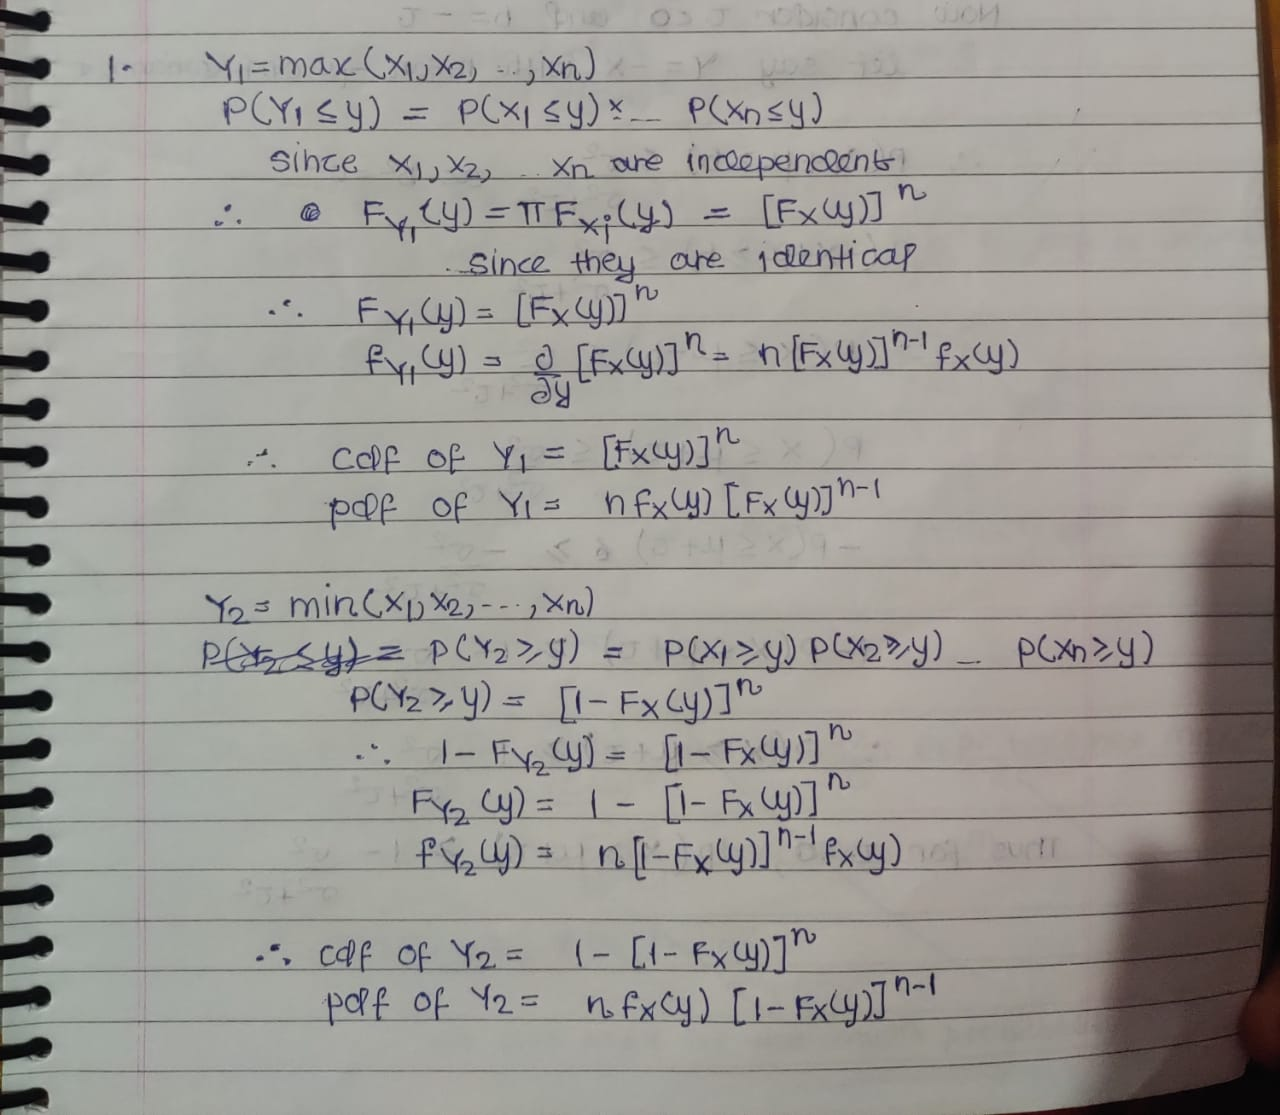
\includegraphics[width=\textwidth, height=\textheight, keepaspectratio]{1.jpeg} \par
\section{Question 2}

\section{Question 3}
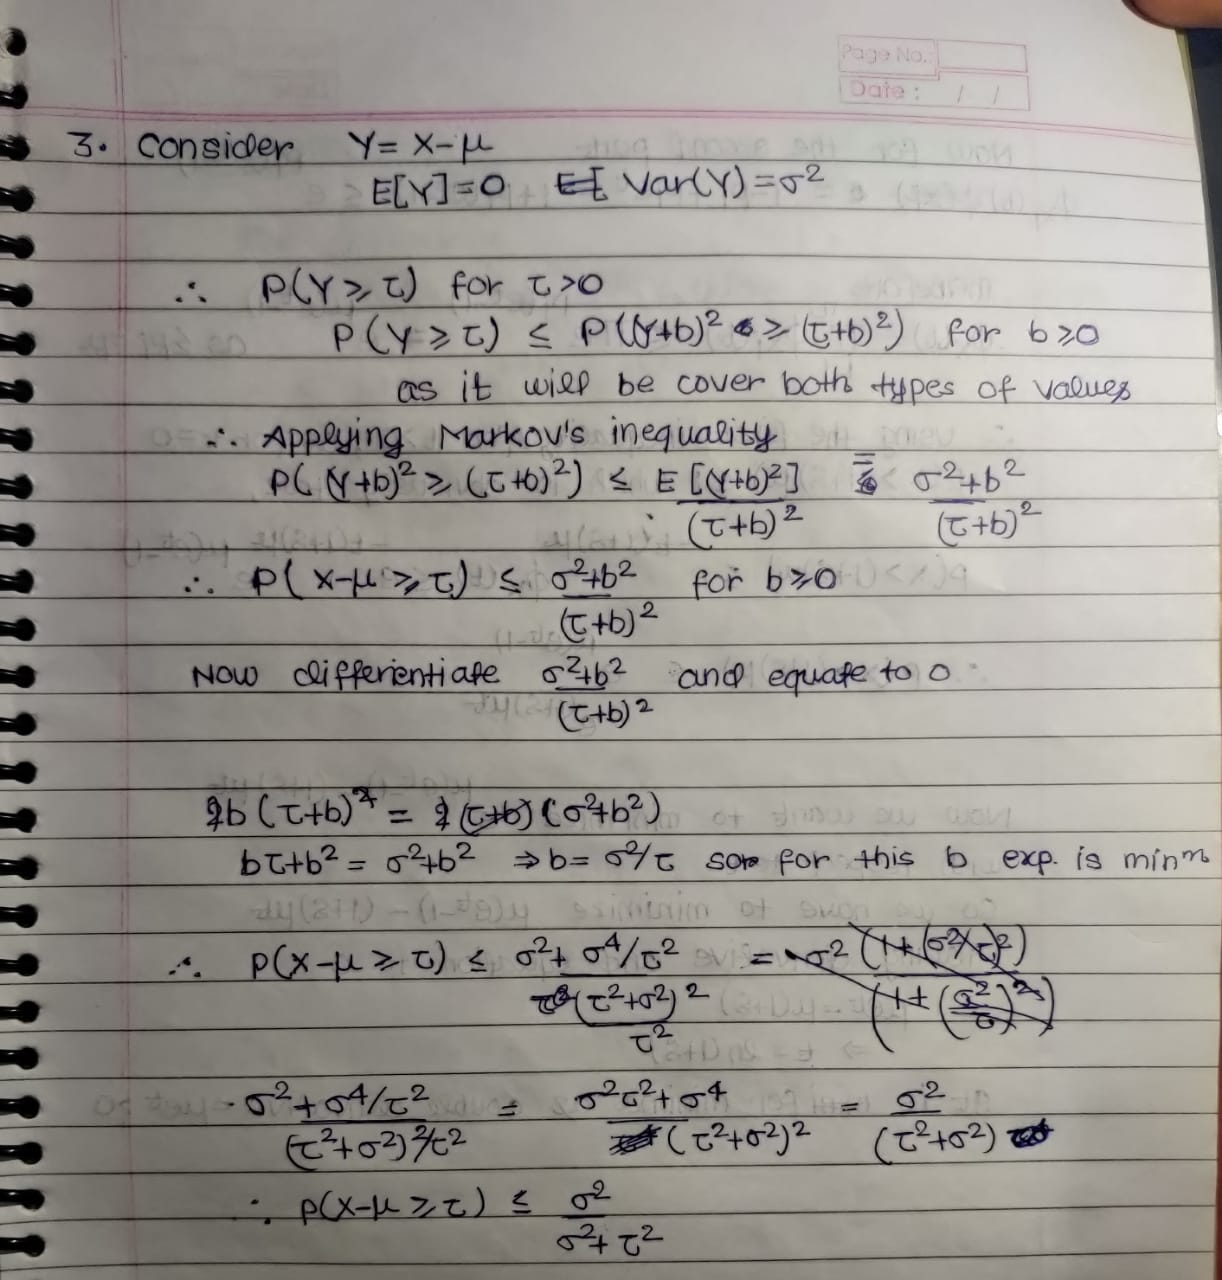
\includegraphics[width=\textwidth, height=\textheight, keepaspectratio]{3a.jpeg} \par
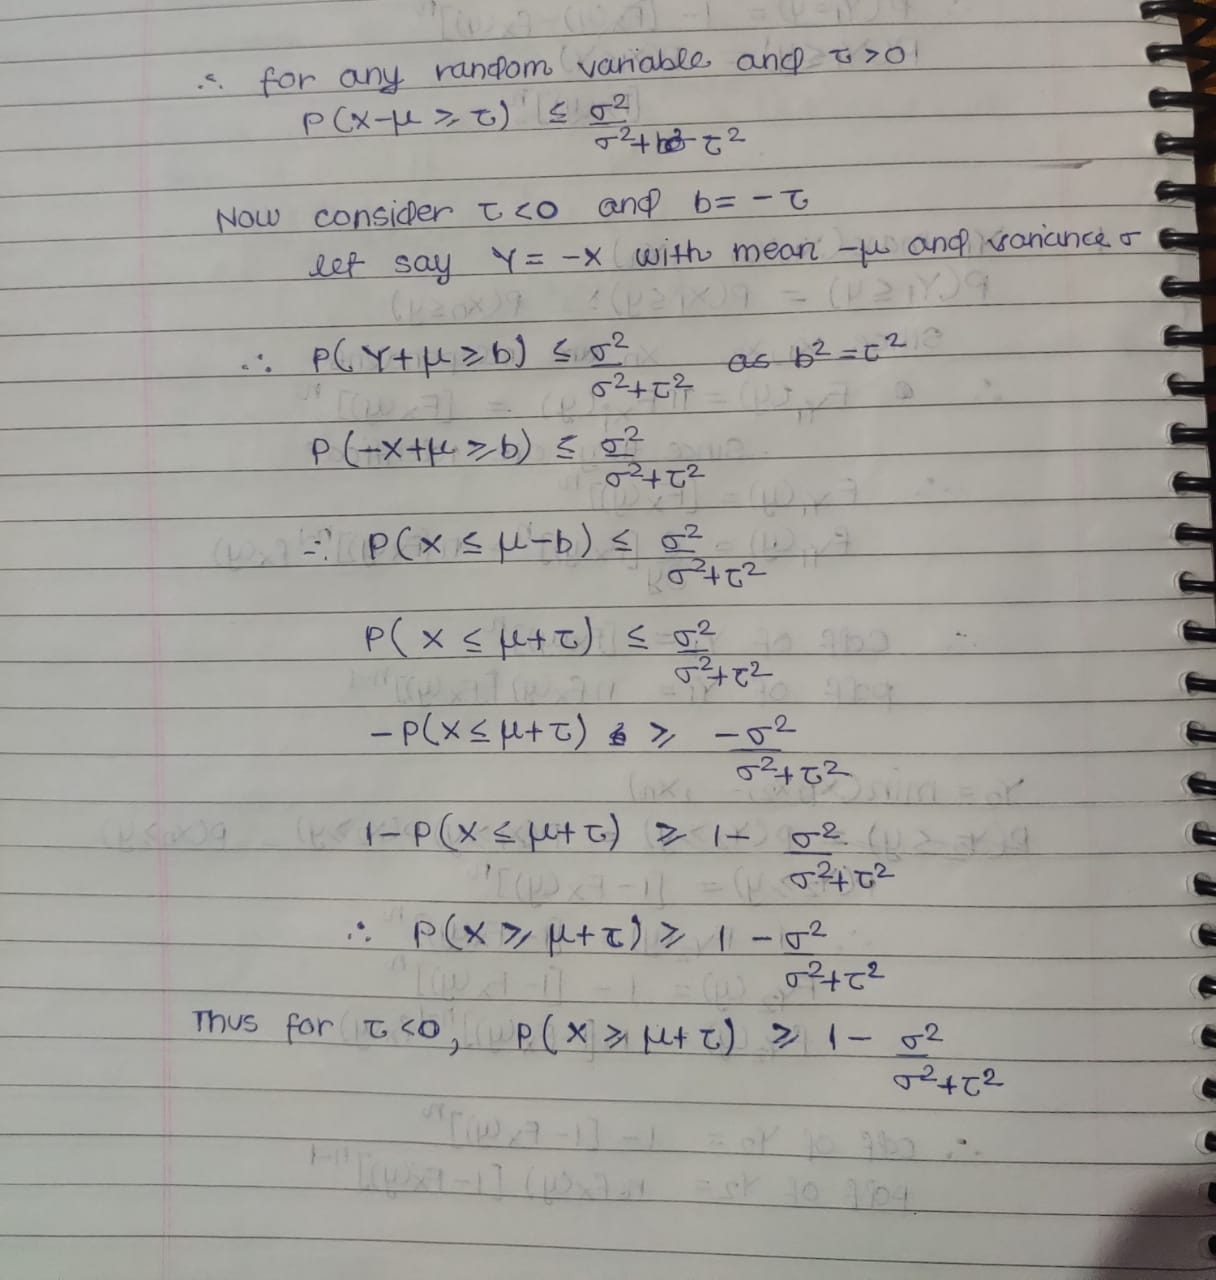
\includegraphics[width=\textwidth, height=\textheight, keepaspectratio]{3b.jpeg}\par
\section{Question 4}
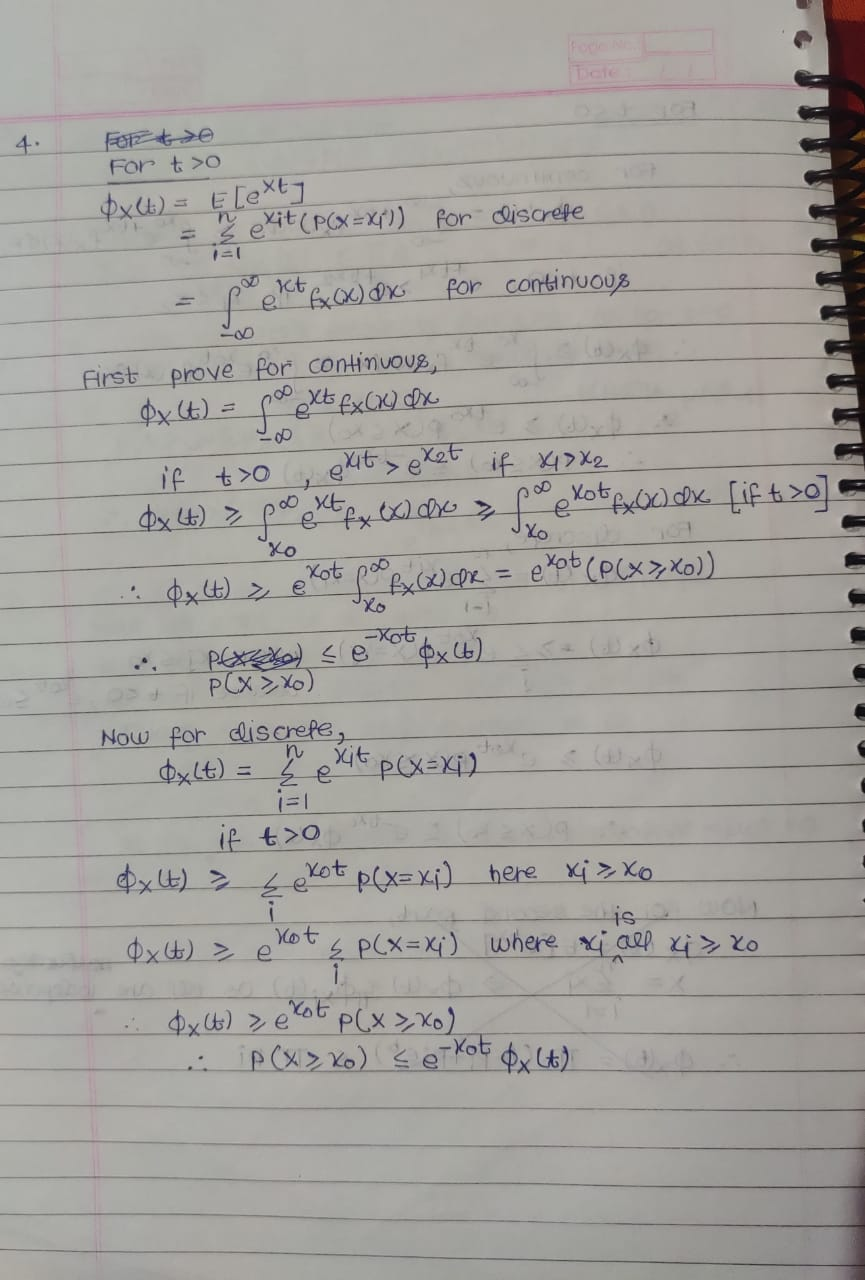
\includegraphics[width=\textwidth, height=\textheight, keepaspectratio]{4a.jpeg} \par
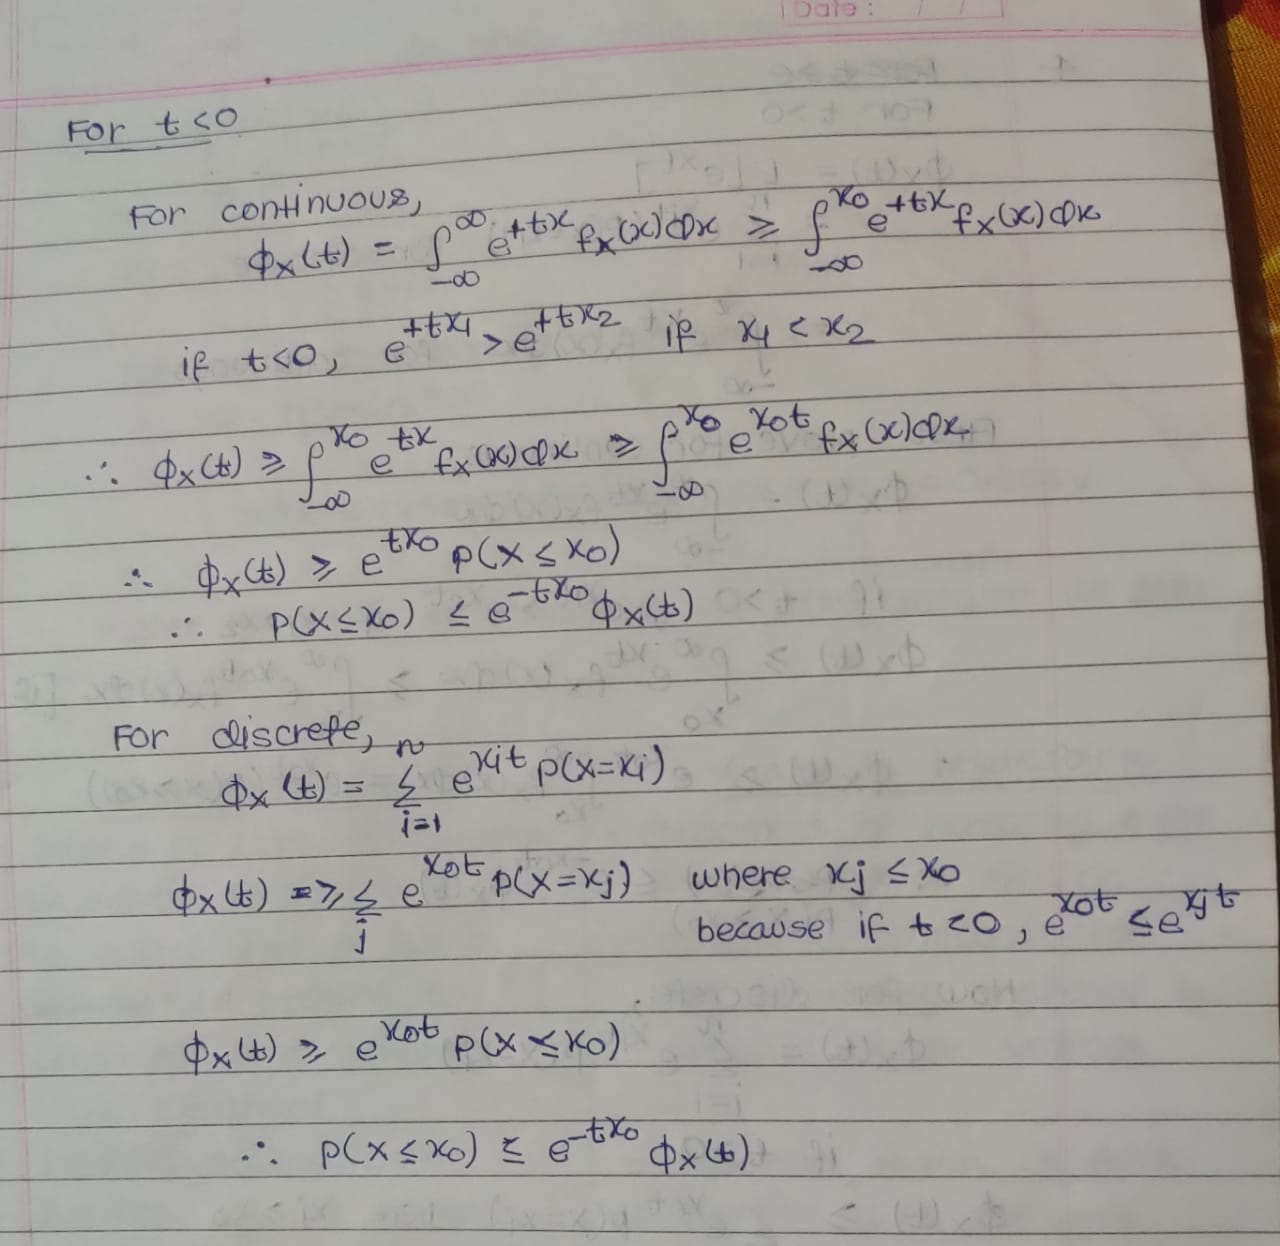
\includegraphics[width=\textwidth, height=\textheight, keepaspectratio]{4b.jpeg} \par
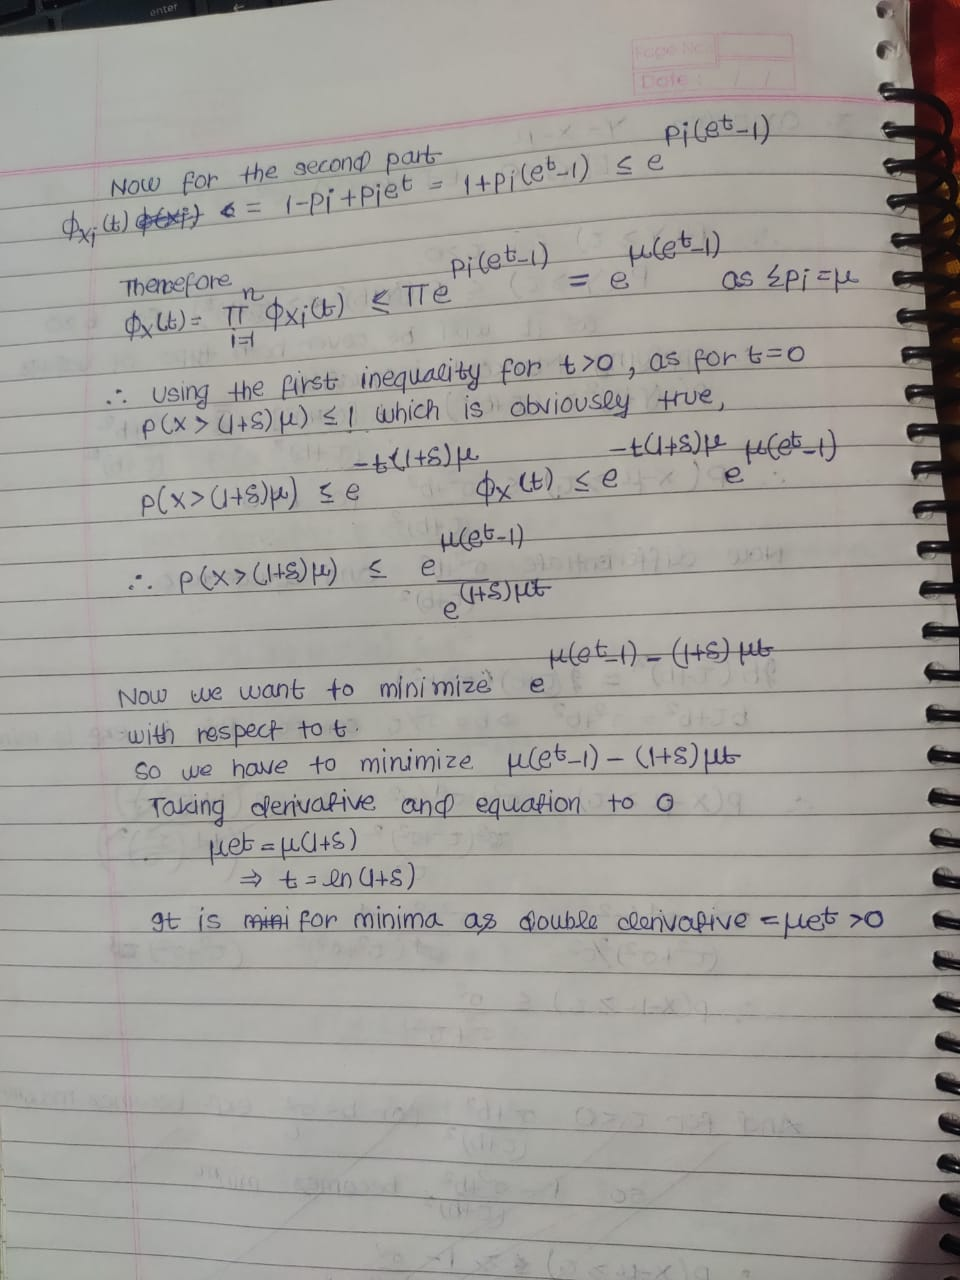
\includegraphics[width=\textwidth, height=\textheight, keepaspectratio]{4c.jpeg} \par
\newpage
\section{Question 5}
Code for this qsn is in file named 'q5.m' \par
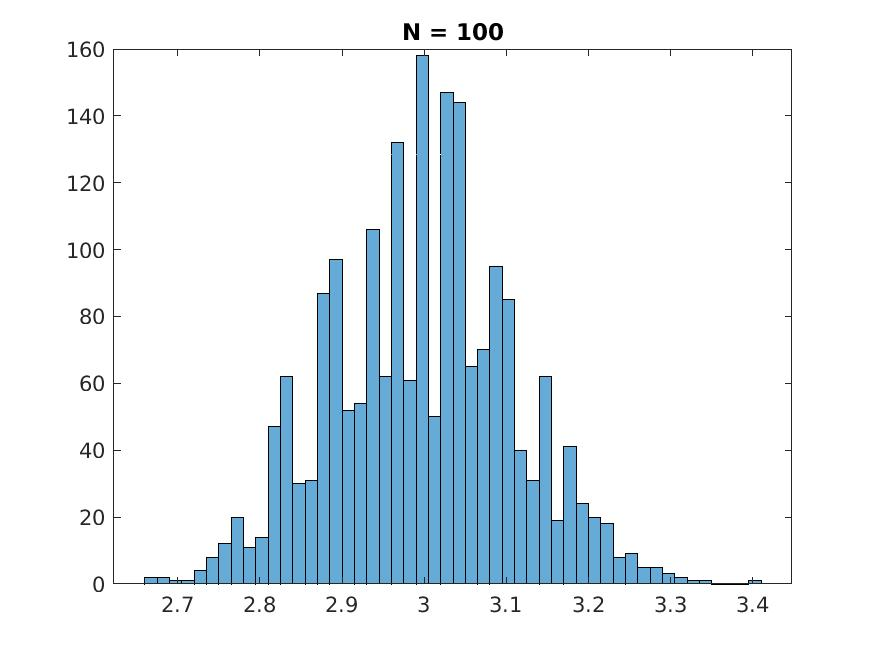
\includegraphics[width=\textwidth, height=\textheight, keepaspectratio]{p1_100.jpg}\par
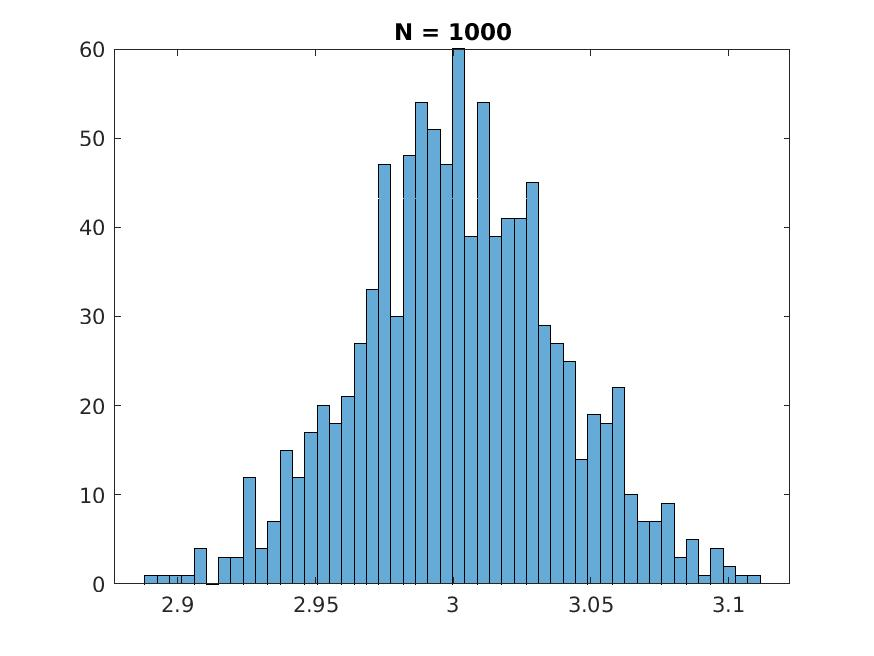
\includegraphics[width=\textwidth, height=\textheight, keepaspectratio]{p1_1000.jpg}\par
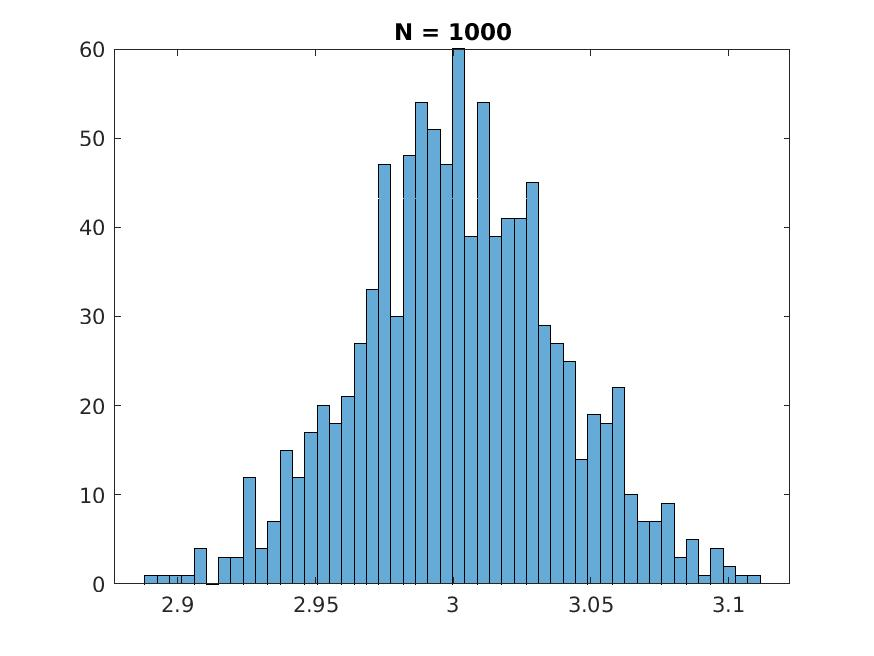
\includegraphics[width=\textwidth, height=\textheight, keepaspectratio]{p1_1000.jpg}\par
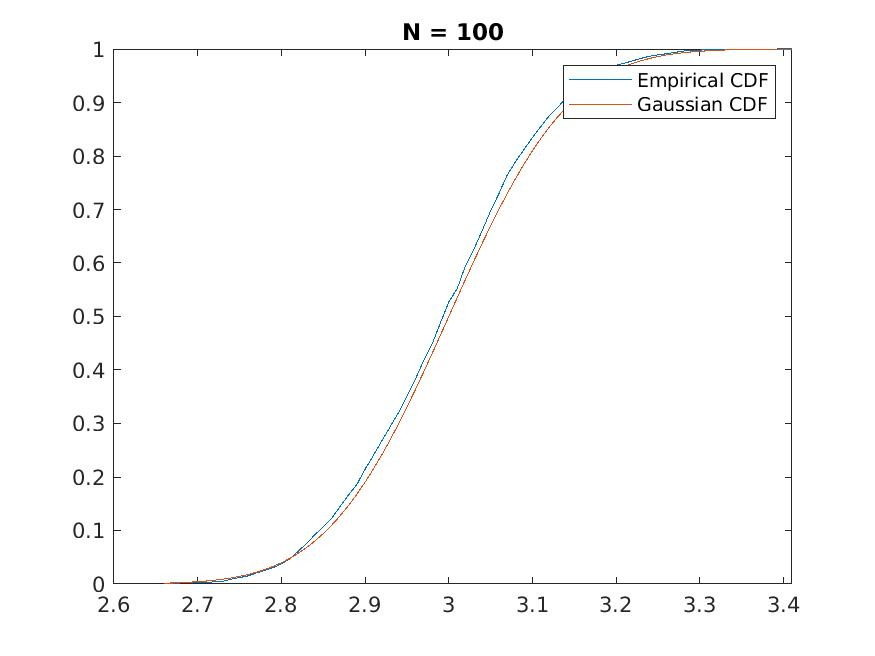
\includegraphics[width=\textwidth, height=\textheight, keepaspectratio]{p2_100.jpg}\par
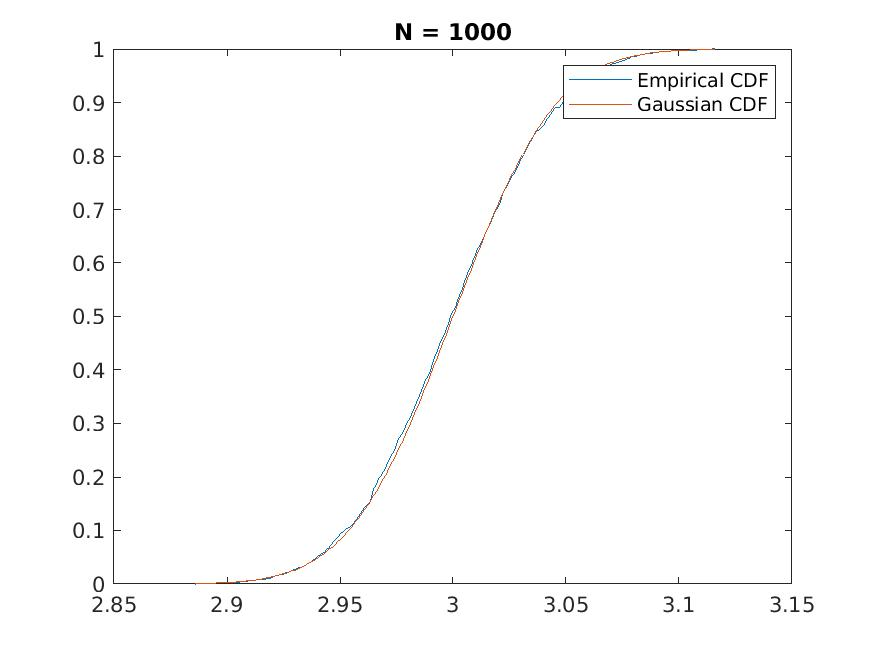
\includegraphics[width=\textwidth, height=\textheight, keepaspectratio]{p2_1000.jpg}\par
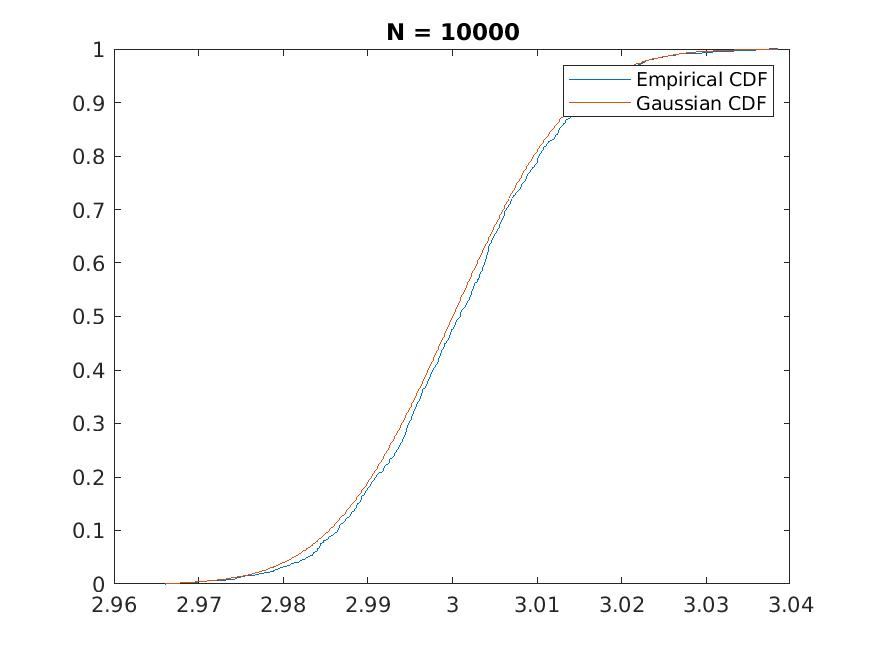
\includegraphics[width=\textwidth, height=\textheight, keepaspectratio]{p2_10000.jpg}\par
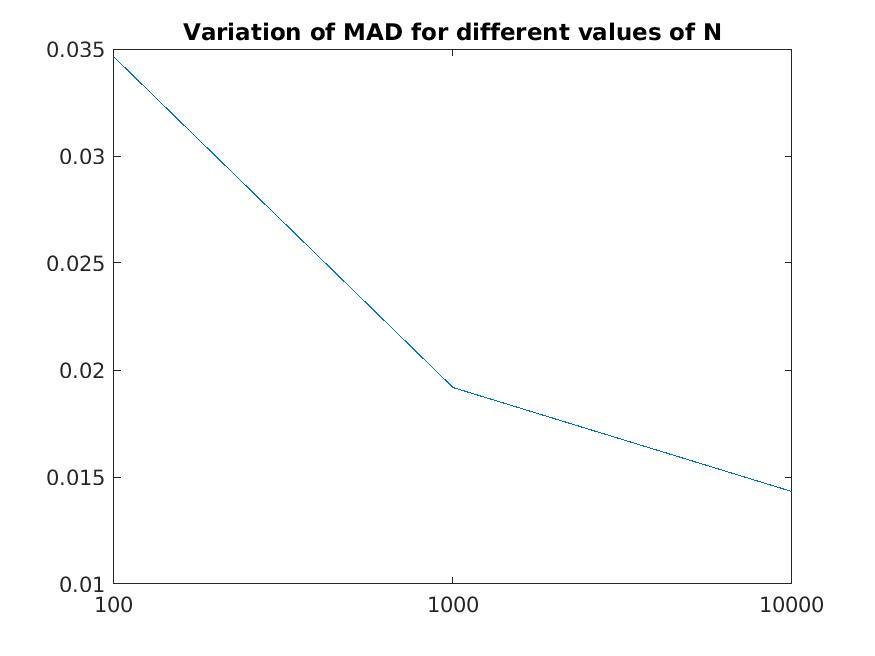
\includegraphics[width=\textwidth, height=\textheight, keepaspectratio]{p3.jpg}\par
\newpage
\section{Question 6}
% \begin{figure}[h!]
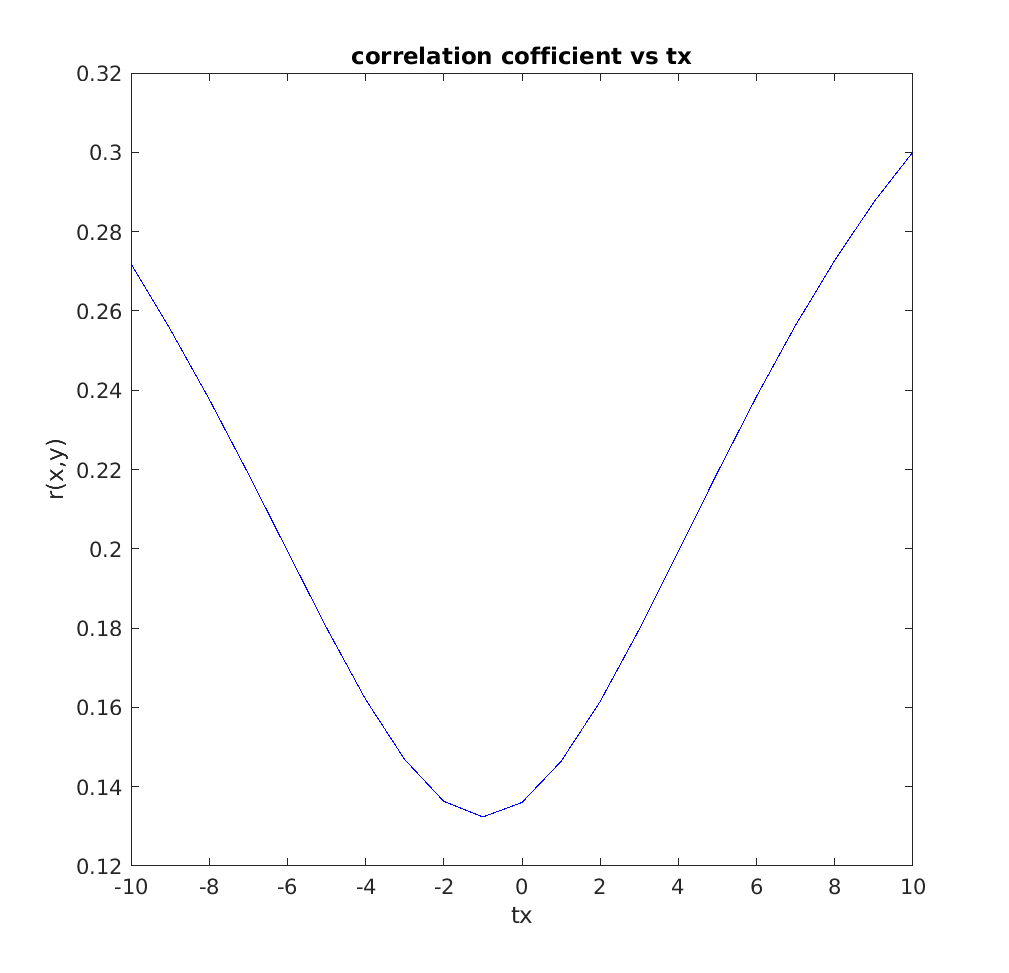
\includegraphics[width=\textwidth, height=\textheight, keepaspectratio]{cor_cof1.png}
\captionof {figure} {This plot correspond to T1.jpg}
% \end{figure}

\begin{figure}[h!]
    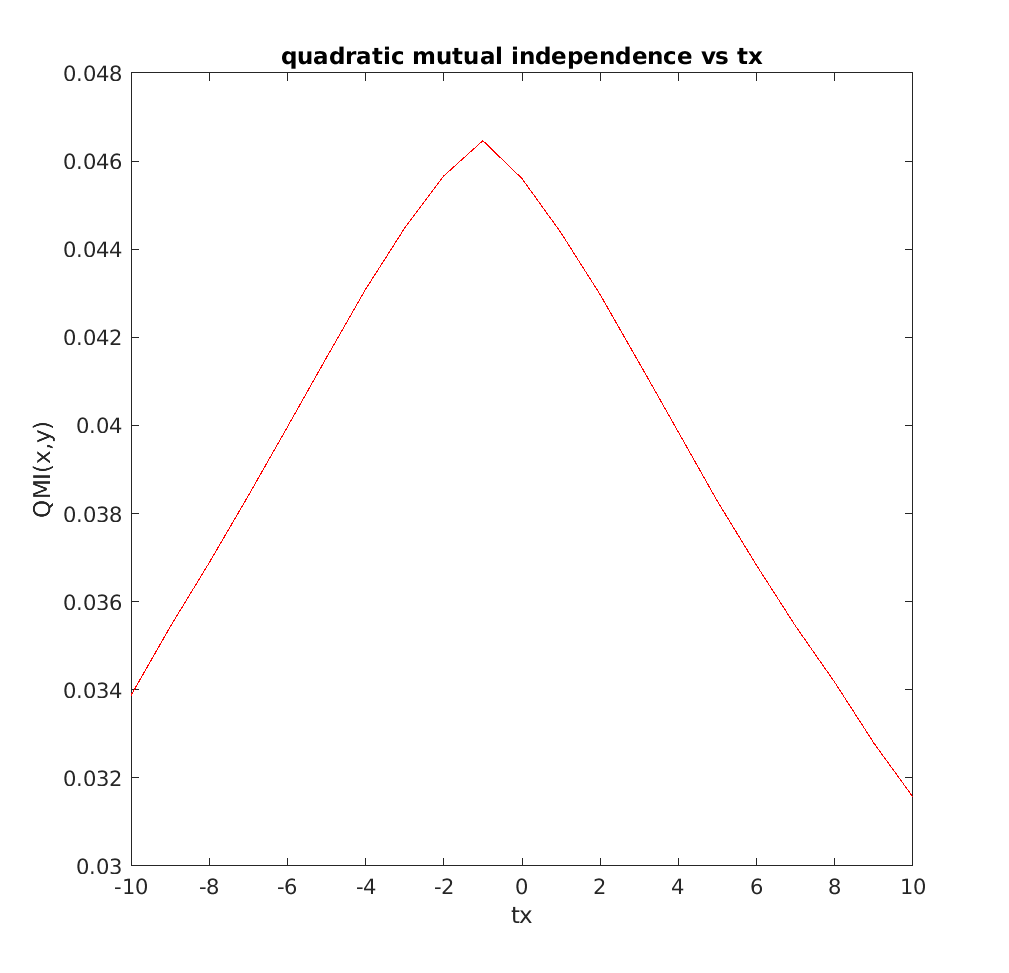
\includegraphics[width=\textwidth, height=\textheight, keepaspectratio]{quadMutInf1.png}
    \caption{This plot correspond to T2.jpg}
\end{figure}

\begin{figure}[h!]
    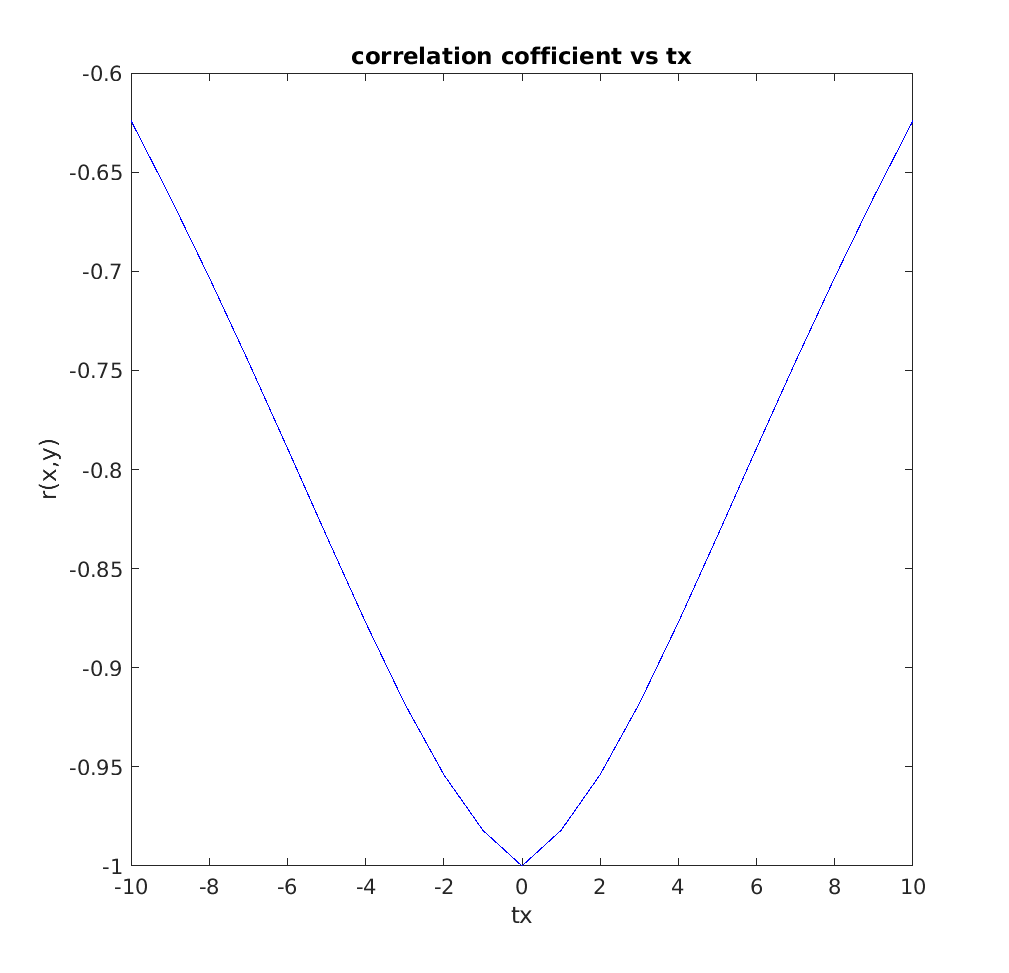
\includegraphics[width=\textwidth, height=\textheight, keepaspectratio]{cor_cof2.png}
    \caption{This plot correspond to T1.jpg and negative of T1.jpg}
\end{figure}

\begin{figure}[h!]
    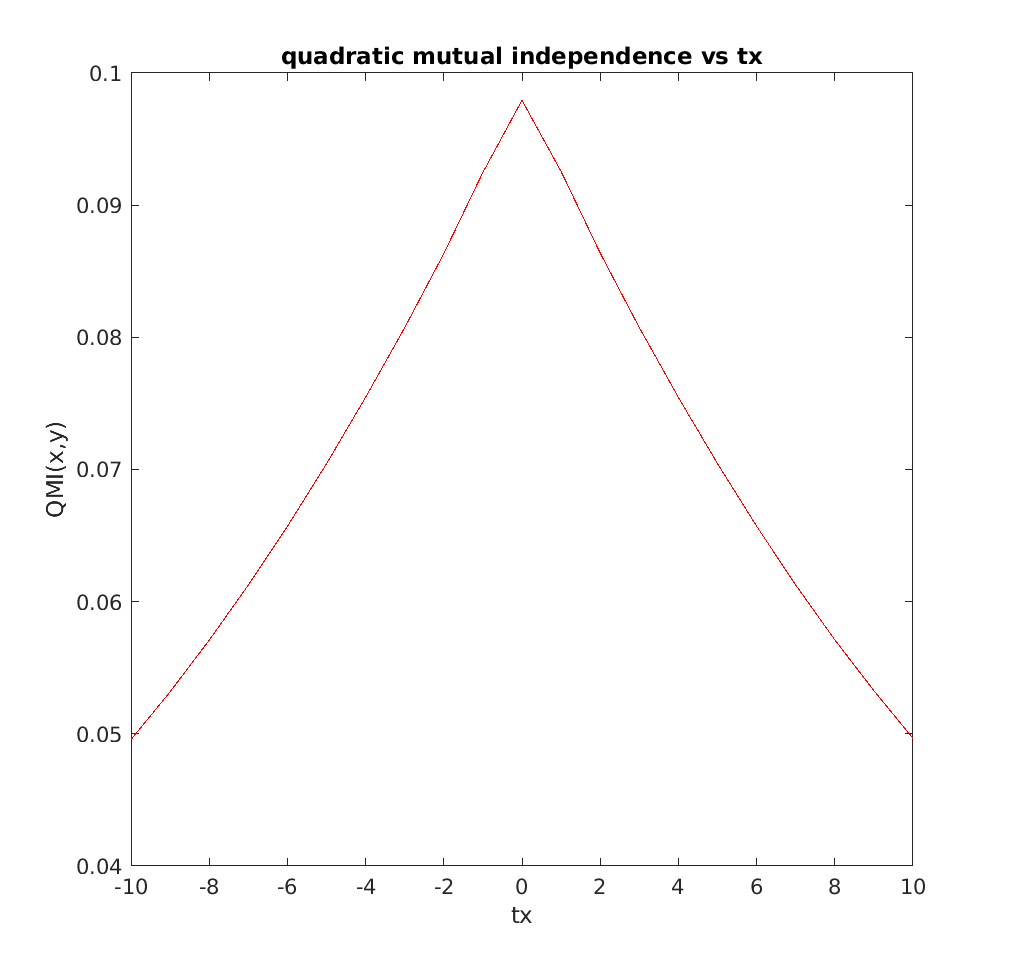
\includegraphics[width=\textwidth, height=\textheight, keepaspectratio]{quadMutInf2.png}
    \caption{This plot correspond to T1.jpg and negative of T1.jpg}
\end{figure}

\newpage



\section{Question 7}
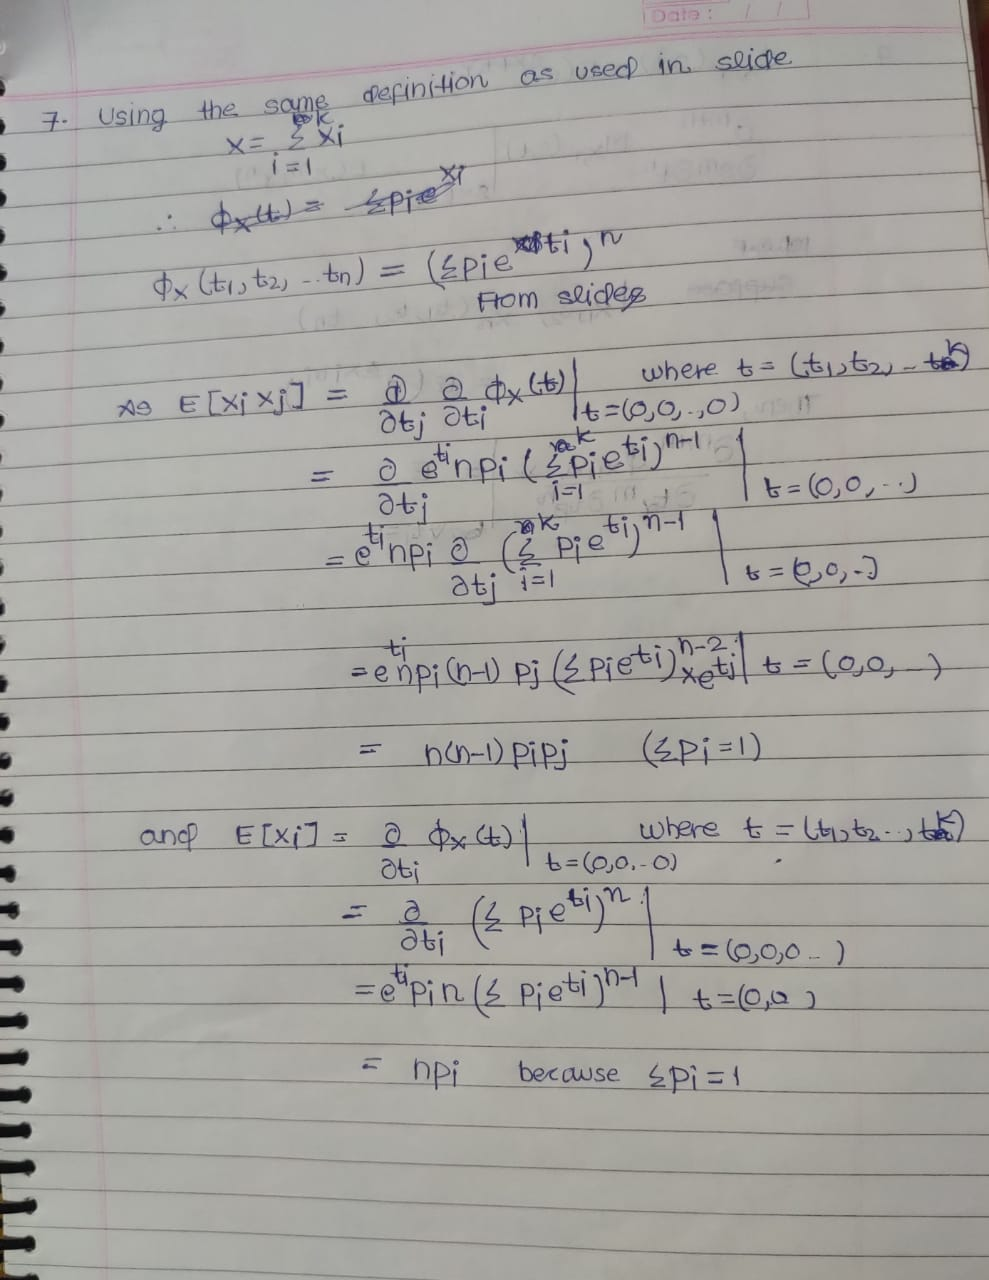
\includegraphics[width=\textwidth, height=\textheight, keepaspectratio]{7a.jpeg}\par
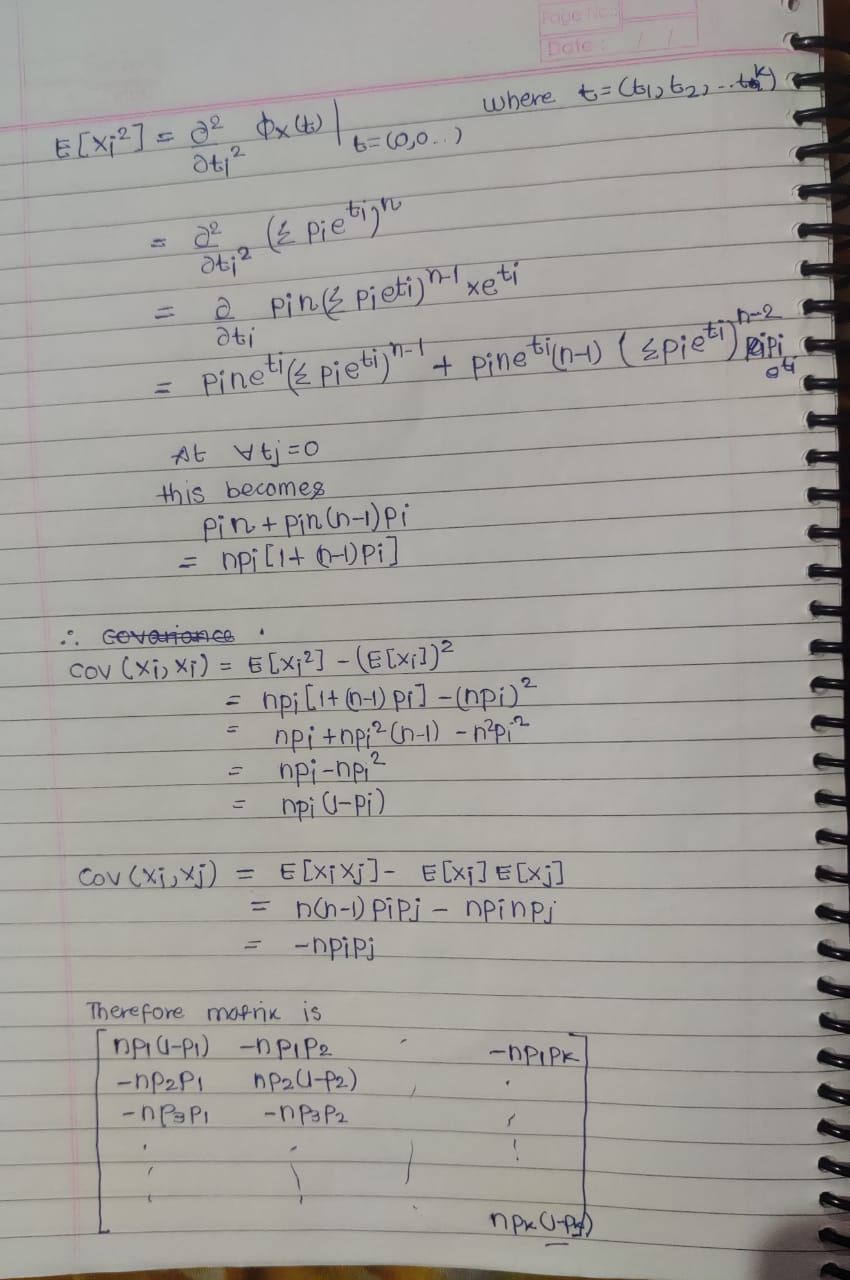
\includegraphics[width=\textwidth, height=\textheight, keepaspectratio]{7b.jpeg}\par
\end{document}